
\documentclass{mpaper}
\usepackage{subfigure}
\usepackage{caption}

\begin{document}

\title{Compact Routing for Today's Internet}
\author{Benas Jonynas}
\matricnum{2133815}

\maketitle

\begin{abstract}
    The Internet has been growing at a rapid rate at the AS level and routing tables have grown alongside it, requiring larger and larger routing tables to ensure that all destinations can be reached. Because of this greater expense is introduced to ISPs who need to continue improving their hardware to maintain quality of service. This paper shows that the Thorup-Zwick compact routing algorithm could be used to reduce the size of routing tables significantly with low path stretch, which could be a potential solution to the scalability issues of the current system.
\end{abstract}

\section{Introduction}

At a high level, the Internet is a collection of independent networks which are connected together. These networks are known as Autonomous Systems (ASes), and they cooperate to transfer data between each other. Currently inter-AS routing is performed using the Border Gateway Protocol (BGP) which was first introduced in 1994 \cite{rfc4271}. BGP uses shortest policy-compliant path routing, which means that the AS path data takes is the shortest possible that adheres to the policy of the owner of the AS. This allows for faster data transfer as fewer ``hops'' are required to route packets from one AS to another. However to be able to route a packet to a destination AS, BGP requires an entry for that AS to be stored in a router's routing table. When BGP was first introduced there were just over 3000 \cite{RIRStats} ASes in the network, today there are over 90,000. Because of this, routing tables have also grown significantly. This is a problem as whole routing tables have to be stored in fast memory in routers to ensure that the next AS in every packet's route can be found quickly. As tables grow larger and larger, more memory is required for routers, leading to more expenses for ISPs and a potential chokepoint for further growth of the Internet. 

One possible alternative to using BGP could be to use a routing protocol based on compact routing algorithms. Compact routing algorithms aim to reduce routing table size by not exposing all ASes to the whole network. This means that the route a node takes might not be the shortest one, but it is cheaper to store the full routing table saving resources for a router. One example of how this is done is through the use of landmark nodes in the Thorup-Zwick (TZ) algorithm \cite{thorup}. Each AS only stores the path to nearby nodes and all of the landmark nodes and each node is assigned to a landmark node that is closest to it. This means that a routing table only needs to store part of the full network yet still retains the ability to route a packet to any required destination. 

This paper's contributions are as follows:
\begin{itemize}
    \item A study of the changes in the topology of the Internet which demonstrates increased connectivity between ASes in the AS graph today
    \item Results demonstrating that k-cores decomposition can be used to produce an effective set of landmarks for the Thorup-Zwick algorithm
    \item Results demonstrating that using the Throup-Zwick algorithm can be used for routing in the AS graph while incurring low path stretch compared to shortest path routing 
\end{itemize}

The rest of this paper is structured as follows:\newline

\textbf{Section 2} provides an overview for the motivations for this project\newline

\textbf{Section 3} provides a more detailed explanation of the TZ algorithm and k-core decomposition. It also presents the data on whether using the k-max shell as a landmark set for TZ satisfies the constraints of the landmark set\newline

\textbf{Section 4 } describes the path stretch produced by using TZ algorithm instead of shortest path routing and shows how this has changed over the last 19 years\newline

\textbf{Section 5} provides an evaluation for the project\newline

\textbf{Section 6} presents the conclusions of the project \newline


\section{Motivation}

A major motivator for adopting compact routing algorithms for inter-AS routing has been the speed at which routing tables are growing. To maintain a high speed of service and be able to process large numbers of requests a router must be able to keep its full routing table in fast memory. This results in increased expense for ISPs as routing tables continue to grow as routers with more and more memory are required. As can be seen in figures 1a and 1b, the size of the network and the number of entries stored in a BGP routing table have grown rapidly over the last 19 years. As this growth continues, ISPs continue to incur more expenses. Furthermore, if the rate of growth increases beyond the rate at which router hardware can be improved, a bottleneck for the growth of the Internet could be created as routers might no longer be able to forward packets as quickly. Therefore an alternative system is needed which would reduce the size of routing tables to ensure that the quality of service within the Internet is preserved. 

\begin{figure*}
  \centering
  \subfigure[the growth in the number of ASes visible to BGPStream between 2001 and 2019 ]{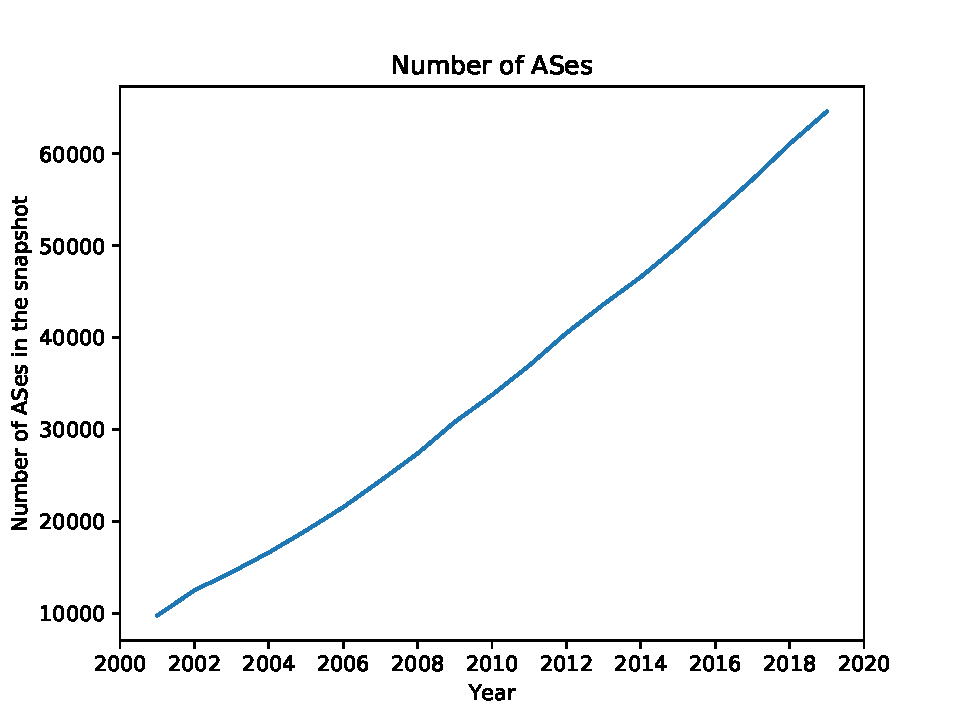
\includegraphics[width=.4\paperwidth]{images/num-nodes-all.pdf}}\hfill
  \subfigure[the growth in the number of entries in BGP routing tables between 2001 and 2019 \cite{CIDR-Report}]{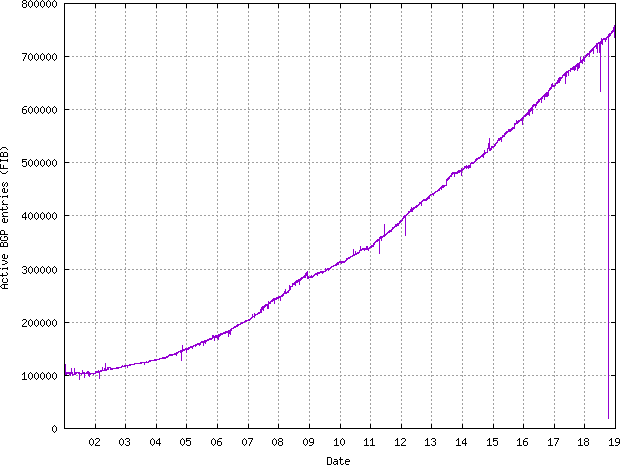
\includegraphics[width=.4\paperwidth]{images/bgpEntries.png}}
  \caption {Growth in the number of AS numbers detected using BGPStream and the number of entries in BGP routing tables}
\end{figure*}

The study in \cite{strowes} examined the effectiveness of using compact routing algorithms for routing in the Internet using the Thorup-Zwick and Brady-Cowen algorithms. It used a series of snapshots of the Internet's topology spanning 11 years to examine the impact that using compact routing algorithms would have on the size of routing tables and path stretch. The results were promising for both algorithms, with the TZ algorithm showing an average path stretch of only 1.09, compared to the worst-case path stretch of 3. This meant that in most cases the path chosen using the TZ algorithm only had a single additional hop compared to the shortest path. The growth observed in routing tables compared to growth in the network was also lower than that of BGP: over the course of the 11 years ``the routing tables have increased in size by 3.5 times; while the graph has [grown] 9.5 times larger''. These results demonstrate that the TZ algorithm was an effective choice for routing in the AS graph.

The study was done in 2012 however, and in the meantime the topology of the Internet has changed. The Internet at the AS level has been observed to grow flatter over the years, with the flattening already being observed by \cite{gill} in 2008. The researchers found that large content providers like Google and Microsoft had begun to by-pass higher tier ISPs in favour of developing their own network infrastructure and setting up direct connections with other ASes. As more networks directly peer with each other, the overall topology grows flatter. This could increase the number of landmark nodes required to maintain short routing paths might increase, reducing the benefits of using compact routing. 

Since the study in \cite{gill}, other research has also found that the AS graph has grown flatter. The study in \cite{carisimo} has investigated the extent to which content providers have become part of the core network of the Internet, which was previously comprised mostly of high tier ISPs. They used the k-cores decomposition technique to identify the ASes at the core of the Internet, which can be associated with the companies the they are registered with. The researchers examined the growth of ``the Big Seven'' content provider networks, including Facebook, Google, and Amazon. They found that each of those networks had ``moved from third-party CDNs'' and their own networks entered nucleus of the Internet. Furthermore, each network had entered the nucleus across all RIRs, and the researchers also found that the `core of the network has been rapidly incorporating content ASes over time.

Another development in the topology of the Internet has been the growth of Internet Exchange Points, or IXPs. IXPs are points where many ASes can peer with each other freely and exchange traffic. Their impact on the network was examined by \cite{gregori}. The researcher used a number of properties such as average neighbour degree and betweenness centrality to determine how important nodes were in the network. This was compared with data from a k-cores decomposition of the network. The researcher found that nodes which participated in IXPs were ``fundamental for inner k-cores'', while nodes which were part of less well connected clusters tended also not to participate in IXPs. Furthermore, the researcher found that a significant number of nodes in the k-max shell were connections which crossed IXPs. This implies that IXPs form an integral part of the core of the network today. This could potentially be beneficial for adopting a compact routing system using the TZ algorithm as it is possible that IXPs could naturally form good landmarks. On the other hand, it is also possible that they could contribute to reducing the benefit of using such a system by increasing the size of the routing table. Therefore, research is required to test whether the changes in the topology of the Internet will have resulted in increased path stretch and/or greater routing table size for a compact routing algorithm, or if compact routing still brings the benefits it did in the past and is still a good alternative for BGP. 

\section{Compact Routing}
\subsection{Thorup-Zwick Algorithm}

The Thorup-Zwick algorithm \cite{thorup} is a compact routing algorithm which utilizes a set of landmark AS addresses to cut down the size of routing tables while maintaining short paths. Routing using the TZ algorithm can be likened to navigating between cities using road signs. For far away destinations, only the major cities will have signs directing towards them. As the destination gets closer the direct path is eventually pointed out by road signs. Similarly, the algorithm uses a set of highly connected landmark nodes which have entries in every node's routing table. Aside from these nodes, each node only contains entries for nodes that are closer to them than any landmark node. This allows for only small routing tables to be stored at each location while preserving the ability to route to any node in the network.

The landmark set is initially composed of a set of nodes chosen at random with a uniform probability for each node to be chosen. Once this initial set is chosen, the clusters for each node are calculated. For a node \textit{u} to be added to the cluster \textit{W$_v$} of node \textit{v}, it must satisfy the following formula:

\[W_v = \{u \in V | d(v,u) < D(A,u)\}\]

where V is the set of all nodes in the graph, $d(v,u)$ is the shortest path distance between $v$ and $u$, and $d(A,u)$ is the distance between $u$ and the landmark node closest to $u$.

Once all nodes have had their cluster calculated, the next step is to check whether any nodes have clusters that are too large. No non-landmark node should have a cluster larger than $4n/s$ where $n$ is the number of nodes in the graph and $s$ is some value chosen when implementing the algorithm. In \cite{thorup} $s$ is $\sqrt{n/log(n)}$ so this is also the value used in this project. If a node has a cluster that is larger than the limit, that node is added to the landmark set and clusters for all nodes are recalculated. This process repeats until no nodes have clusters which are larger than the limit. 

Once the clustering process is complete and the landmark set is finalized, the routing tables for the nodes are done. A given node's routing table would only contain entries for the nodes in its cluster and the landmark nodes. Routing is done by using a node's address and its closest landmark. If the destination node is present in the current node's cluster, that node is able to route the packet directly to the destination by the shortest path. Otherwise, the packet will be forwarded towards the landmark closest to the destination. This allows the TZ algorithm to heavily reduce the size of routing tables as the table only requires entries for the nodes closest to it and the landmark set which is much smaller then the whole graph.
 
\subsection{K-core decomposition}

K-core decomposition is a technique which can be used to find the set of nodes with the highest connectivity in a graph. The way this is done is by stripping away outer k-shells of nodes with fewer connections. A k-shell is composed of nodes which have k or more connections to other nodes. For example the k-0 shell encompasses the entire graph, the k-1 shell would not include nodes which are isolated without any connections and the k-2 shell would not include leaf nodes with only a single connection to the rest of the graph. Following this, the k-max shell or the k-core would only include those nodes which have the highest number of connections within the graph.

As the landmark nodes in a TZ based routing system would be nodes accessible to the whole network, it would make sense for them to also be the most highly connected nodes. Because of this, nodes from the k-core set could be a good choice as landmark nodes. This idea was also examined in \cite{strowes} who found that in almost all of the samples when the k-max shell was used only a single iteration of the algorithm was required to calculate the clusters for each node. This might mean that routing through these nodes naturally follows the shortest paths. Furthermore, the research found that 70\% of nodes in a k-max shell in a snapshot were still present 3 years later. This would provide greater stability when routing using TZ as fewer landmarks would have to be recalculated. 

\subsection{Internet Topology Data}
For the purposes of the project, snapshots of the AS graph had to be gathered. This was done using BGPStream, a tool which aggregates BGP routing table data from the Route Views and RIPE RIS projects. Both Route Views and RIPE RIS gather topology data using a number of collectors. Collectors advertise themselves to nearby routers as ASes which offer tranit for traffic. Because of this, routers will advertise their routing data with the collectors. With a larger number of collectors, more connections can be discovered as paths from other locations are likely to follow a different path. This can be seen in figures 2a and 2b, which demonstrate the difference between using a smaller subset of the 15 oldest collectors in the two projects and using all collectors available, the number of which grows to 46 at the time the project was done. As can be seen in the figures, there is very little difference between the number of ASes discovered when using the full collector set and a partial one. However, the number of connections discovered grows significantly as more collectors are added.

\begin{figure*}
  \centering
  \subfigure[the number of ASes discovered ]{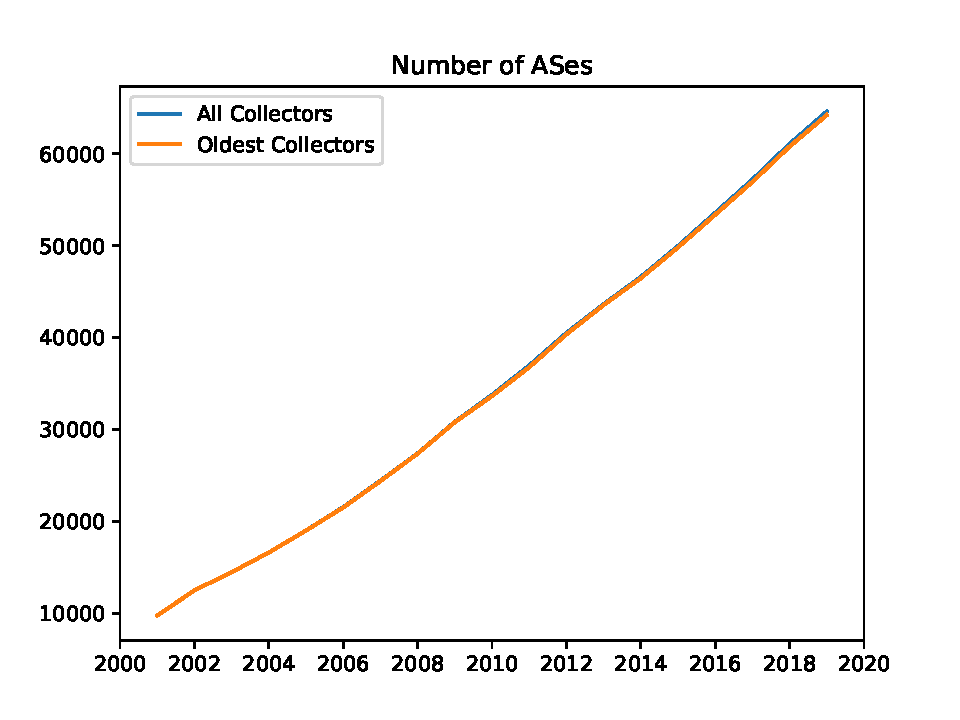
\includegraphics[width=.4\paperwidth]{images/num-nodes.pdf}}\hfill
  \subfigure[the number of connections between ASes discovered  ]{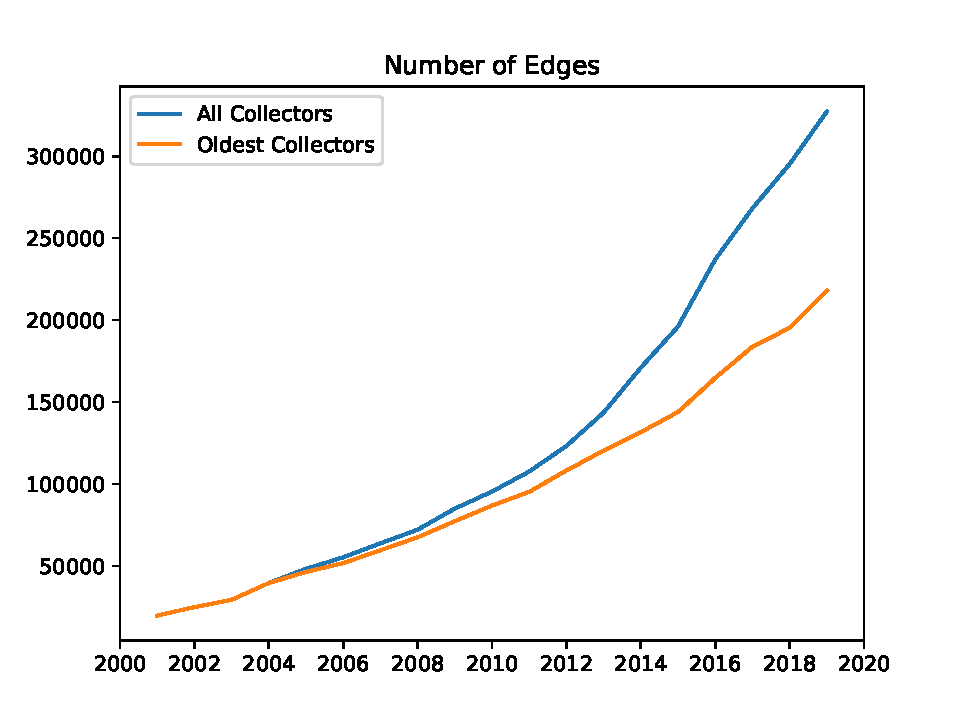
\includegraphics[width=.4\paperwidth]{images/num_edges.pdf}}\hfill
  \caption{The difference in number of ASes and connections between them discovered when using the set of oldest collectors and all available collectors}
\end{figure*}

The snapshots used for the project spanned 19 years, with the first being from 1st January 2001 and the last being from 1st January 2019. The snapshots were composed of data gathered from RIB dumps from all available collectors between the two projects. This was done to gain gather data about the highest number of nodes and edges that can be seen within the network. Furthermore, a duration of 8 hours was used for the time frame over which RIB data was to be gathered. This was to account for the fact that the RIPE RIS project collectors dump RIBs every 8 hours. Setting a time frame longer than the duration between dumps allows us to account for the fact that connections might been down during the time RIB data was last dumped and come back up in the intervening time. A longer time frame was not chosen to reduce the time each data gathering run took.

Snapshot data was gathered from the ``as-path'' field in each entry in a RIB. In BGPStream data the as-path field contains a list of ASes which compose the path from a destination to the collector. In most cases these nodes are in the order which is used to reach the destination node. Because of this the edges for the AS graph are derived from pairs of adjacent nodes in as-path fields with AS numbers being used as node IDs. However some ASes choose to obscure the exact path between different nodes and provide their data as an AS set. While these sets contain all the ASes in the path, the order is not guaranteed to be correct. Across all snapshots the number of nodes in AS sets varies between 0.640\% and 0.462\% with an average of 0.240\% of nodes in a snapshot being part of an AS set. For the sake of completeness, it was assumed that nodes in AS sets are recorded in the correct sequence and edges were created in the order that the AS numbers appear in an as-path. Once all RIB entries have been read and the graph is fully constructed, it is saved into a file as a list of node pairs identifying each edge in the graph.

The data gathered for the project also provides some insight into the topology of the AS graph. Figure 3 shows the percentage for each path length across the different snapshots. It can be seen that aside from one snapshot, the shape of the graph has not changed a great deal. The main differences that can be observed are an increase in the number of paths that are of lengths 4 and 5 and a small decline in paths of greater lengths than this. In addition, the number of paths of length greater than 10 has increased in the later samples, but the proportion of that increase compared to the growth in the rest of the graph is negligible. 

\begin{figure*}
    \centering
    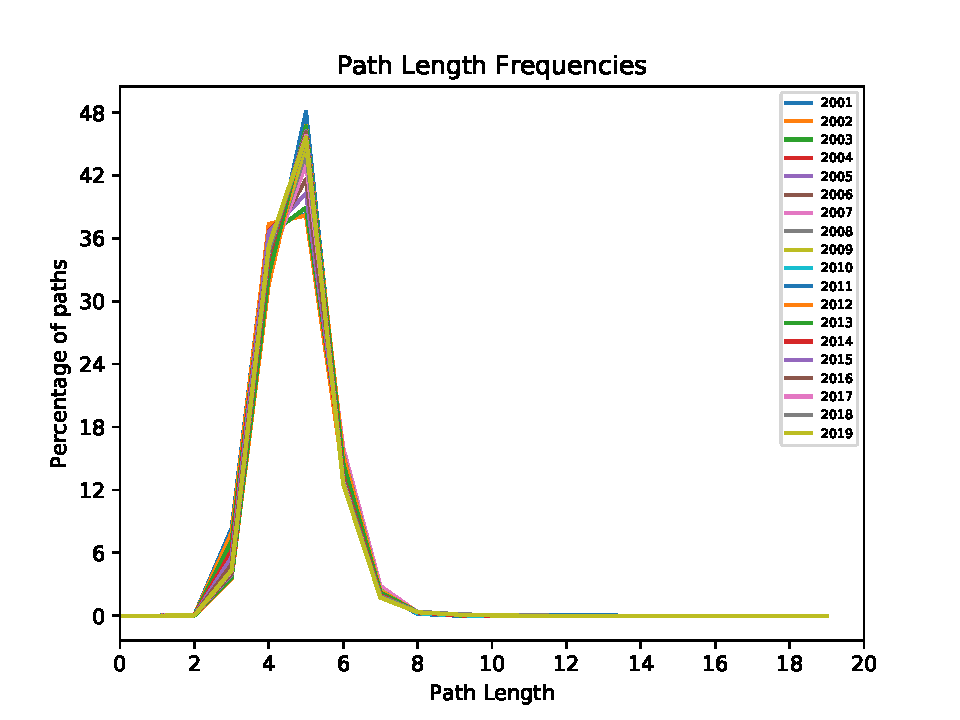
\includegraphics{images/path-frequencies.pdf}
    \caption{Numbers of nodes with different degrees of connectivity}
    \captionsetup{justification=centering}
\end{figure*}

\begin{figure*}
  \centering
  \subfigure[the percentage of snapshots with clusters greater than 0 ]{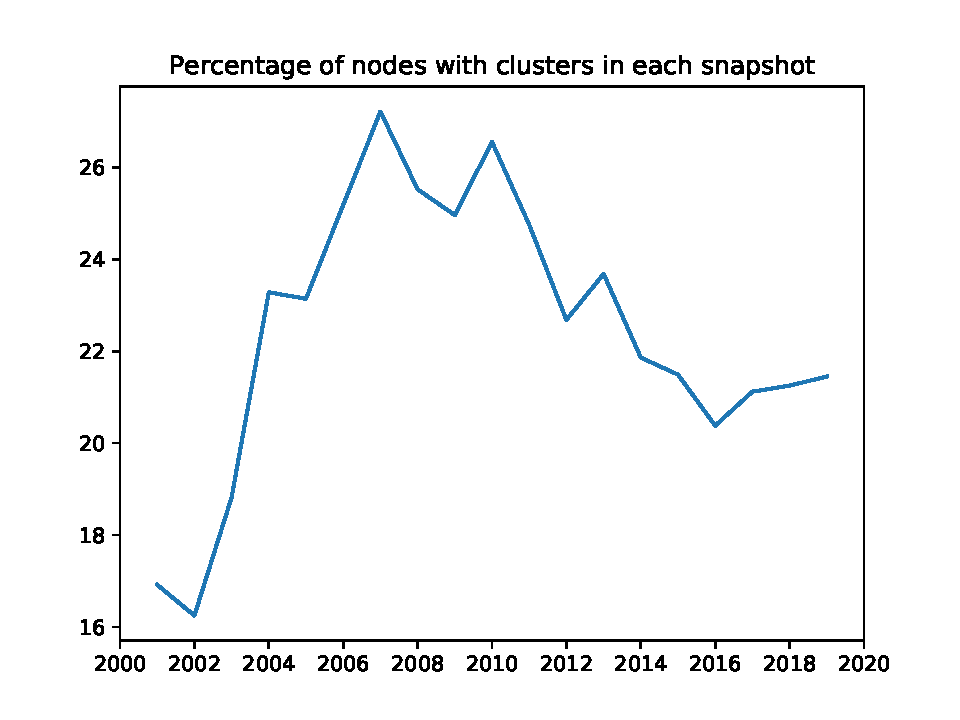
\includegraphics[width=.4\paperwidth]{images/nodes-with-clusters.pdf}}\hfill
  \subfigure[the average cluster size of nodes that have a cluster size greater than 0 ]{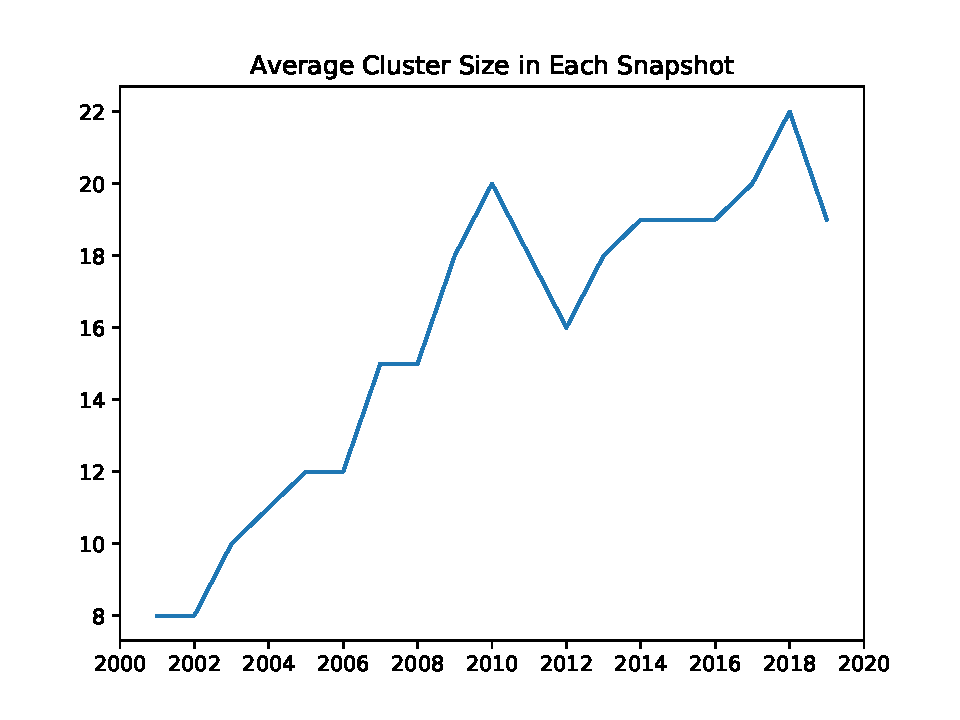
\includegraphics[width=.4\paperwidth]{images/average-cluster-size.pdf}}\hfill
  \caption{Cluster data for each snapshot}
\end{figure*}

\subsection{Using k-core as a landmark set}
Part of this project has been to investigate whether the k-max shell of the network provides an effective choice of landmarks for the TZ algorithm. This was done by first importing the snapshot data. The data is at this point contained in a file as a list of node pairs representing connections between ASes. Each AS number is treated as a unique node ID and all connections are between adjacent ASes with an edge weight of 1. The created graph did not have any self-loops and was undirected.

Once the graph was imported, the next step was to calculate the k-max core of the graph. This was done using an inbuilt method of the NetworkX library. For all snapshots the k-cores were calculated until a core of at least size $4\sqrt{nlog(n)}$ was found. As seen in figure 6, the size of the k-max was always a fraction of the size of the total graph and significantly smaller than the $s$ value for each snapshot. 

With the k-cores calculated, each node's cluster was calculated using the k-max shell as the initial landmark set. First, for each node in the graph the shortest paths to all other nodes were calculated using Djikstra's algorithm, and these paths were recorded in a dictionary. Then this dictionary was used to find the paths from the current node to each landmark node. In addition, the ID of the landmark closest to the current node and the length of the path to it were recorded. Following this, the shortest path distances to all other nodes in the network were checked to see if any were shorter than the path length to the closest landmark. Calculating the distance to the current node's nearest landmark and adding the current node to the clusters of each other node that was closer than the landmark required fewer calculations to find the shortest path to the current node's nearest landmark as it only needed to be done once. In the other case where the distance to each node from the current one is calculated and then the shortest path distance for each destination and their landmark is calculated would require a shortest path calculation for every destination, which would significantly increase the running time of the program. 

\subsection{Results}

Once all clusters were calculated, their size was checked against the limit for that snapshot, $4\sqrt{nlog(n)}$. If any clusters were larger, they would be added to the landmark set and the clustering process would be iterated upon until no nodes had clusters larger than the size limit. It was found that when using the k-max set as the starting landmark set, none of the snapshots had nodes which violated the size constraint. This meant that only a single run of the clustering algorithm was required to establish the clusters for all nodes. These finding were also consistent with the findings of \cite{strowes}. 

Figures 4 and 5 present some additional information about the node clusters produced using the k-max set as the landmark set. Figure 4 shows the percentage of nodes in a snapshot that had a cluster. An increase can be seen between the years 2005 and 2012, but following that period the portion of nodes with clusters falls again. In a flattening Internet topology one would expect the percentage of nodes with clusters to increase as nodes become more interconnected and it becomes easier to travel directly between nodes. However a possible explanation for this decrease is the increased prevalence of IXPs. IXPs tend to have a higher connectivity by their nature, which makes it likely that they will be included in the landmark set and that many shortest paths will pass though them. Therefore as more IXPs are added to the landmark set and routing through them becomes more consistent, other nodes are less likely to provide a shorter path to another node.

Figure 5 presents the average cluster size for nodes that do have a cluster. This size can be seen to consistently increase over the years, which indicates that nodes are still becoming increasingly well connected even outside of the core of the network. This does provide evidence for the idea that the topology of the AS graph is getting flatter as the connectivity of nodes is clearly seen to increase.

\begin{figure*}
    \centering
    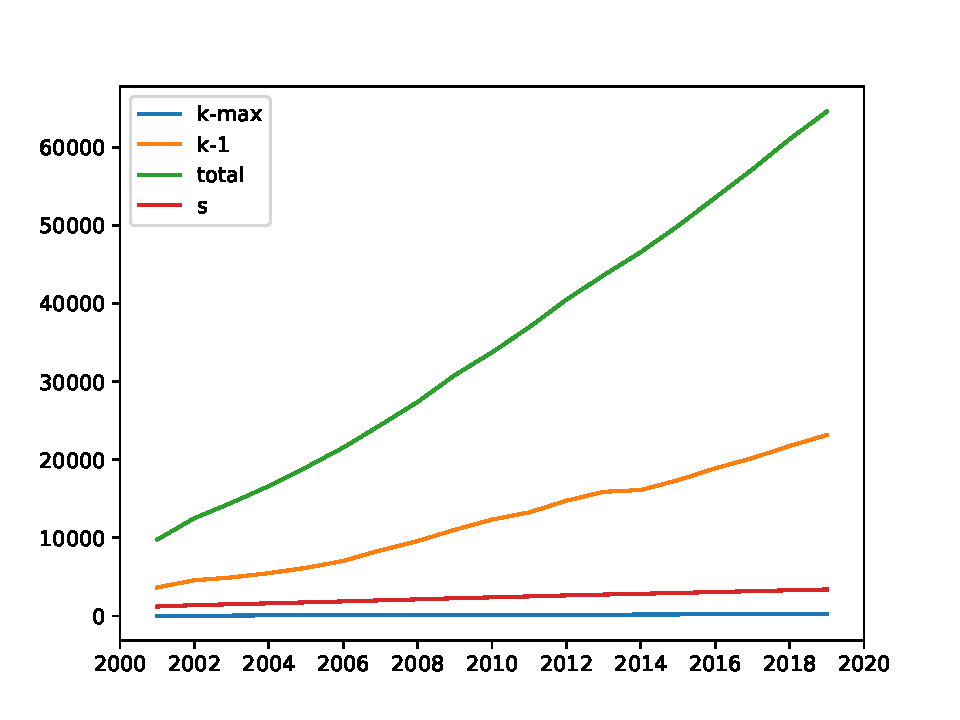
\includegraphics{images/k-cores.pdf}
    \caption{The sizes of k-max, k+1, and $s$ and the total number of nodes in each snapshot}
\end{figure*}

\begin{figure*}
  \centering
  \subfigure[Average shortest path length for each year using TZ routing]{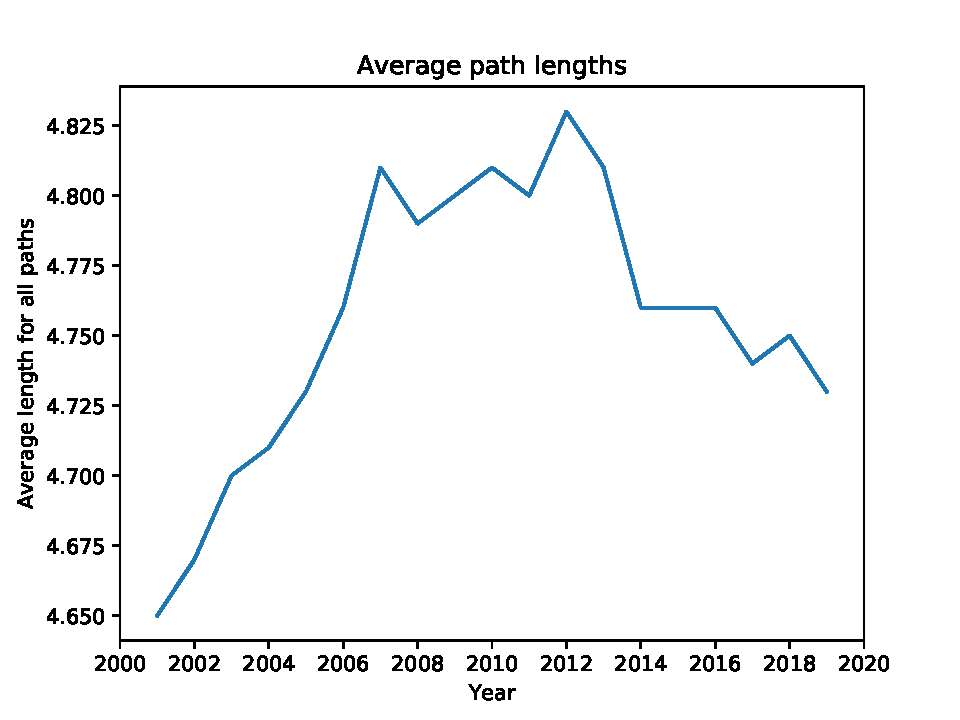
\includegraphics[width=.4\paperwidth]{images/path-averages.pdf}}\hfill
  \subfigure[the average path stretch for each snapshot using TZ routing ]{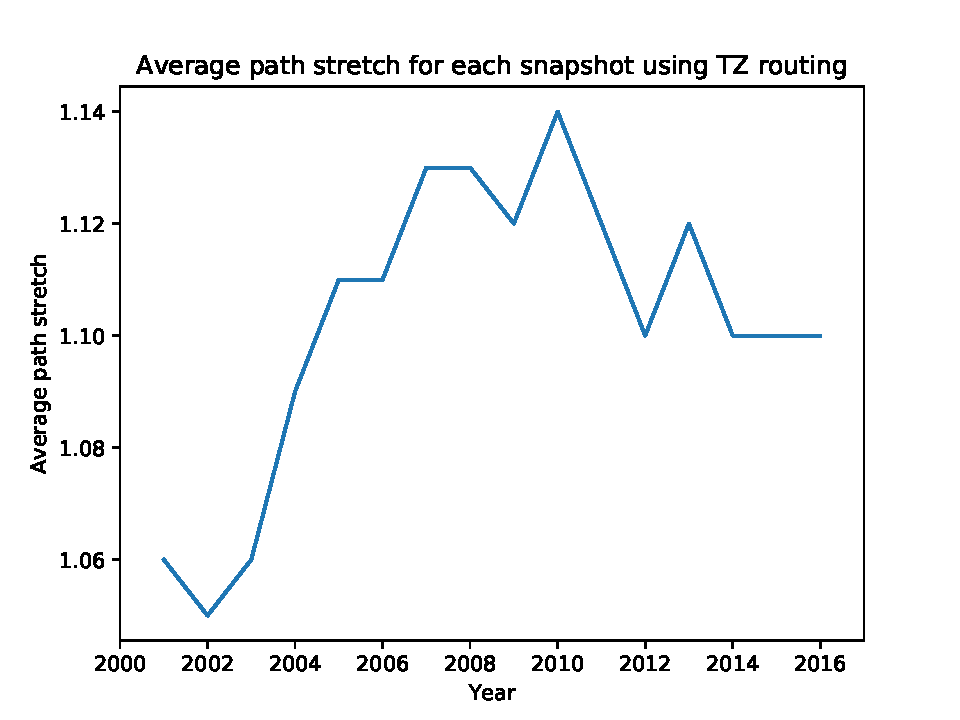
\includegraphics[width=.4\paperwidth]{images/path-stretch.pdf}}\hfill
\end{figure*}

\section{Path Stretch using the TZ algorithm}
\subsection{Methodology}
The final part of this project was to calculate the path stretch between using shortest path routing and TZ routing. Firstly, the graph described previously, the landmark set, and the clusters for each node were imported from file. Following this, all nodes had the shortest path to all landmarks calculated once again. Then 1\% of nodes in the graph were chosen at random to serve as a sample. Calculating the path stretch for every node in the graph would be very time consuming, especially for the later snapshots. Each of the chosen nodes had the shortest paths to all other nodes calculated using Djikstra's algorithm to serve as a baseline data set. 

Following this, each node had its distance to each other node calculated using the landmark set of the TZ algorithm. First, the distance from the current node to the landmark closest to the destination node found using the dictionary holding shortest paths already calculated for the current node. Then the cluster of each node on the way to that landmark was checked. If an entry for the destination node $u$ was wound in the cluster of a node $c$, then the TZ path from node $s$ to node $u$ was calculated as:
\[ D(s,u) = D(s,c) + D(c,u)\]

where $D(s,u)$ is the shortest path distance between the source and the destination nodes, $D(s,c)$ is the shortest path distance between the source node and the node with the destination node in its cluster and $D(c,u)$ is the shortest path distance between the node with the destination in its cluster and the destination node.

If no nodes were found between the source node $s$ and the landmark node closest to the destination $l$, then the landmark node must be part of the shortest path between $s$ and $u$. In that case, the distance between the source and destination nodes was calculated as:

\[ D(s,u) = D(s,l) + D(l,u)\]

where $D(s,u)$ is the distance between the source and destination nodes, $D(s,l)$ is the shortest path distance from the source node to the landmark node closest to the destination and $D(l,u)$ is the shortest path distance from the landmark node to the destination node. The path stretch for each path was calculated as 

\[ Stretch = 1 / D(Shortest Path) * D(TZ Path)\]

Finally the path stretch for each value was added to a total and an average path stretch was produced.
\subsection{Results}

The average path stretch for each snapshot can be seen in Figure 6. It can be seen that the average path stretch has stayed relatively constant over the years and has been consistently low. According to \cite{thorup}, the worst case path stretch for the TZ algorithm is 3. The results of this project show that when applied to the AS graph, the TZ algorithm produces a much lower path stretch than the worst case and is therefore a suitable choice for routing in the AS graph today. 


\section{Evaluation}
This project has succesfully shown that the TZ algorithm can be effectively used to route in the AS graph, requiring a small landmark set and producing low path stretch. However, the project has a number of limitations.

The first is the way the AS graph is modelled. The graph used in the project is an undirected graph where all edges between adjacent nodes have a weight of 1. This could skew the results of the project as edges in the actual AS graph have direction as some ASes allow transit of traffic for some other networks but others do not. The fact that an undirected graph was used could have reduced the average path stretch as paths become available which do not exist in the real AS graph. Furthermore, AS policy has a significant impact on routing decisions. Depending on one AS's relationship to another it might allow traffic through freely, favour some ASes over others or not allow traffic from particular ASes through at all. This project has made no effort to account for the impact of AS policy which when accounted for might introduce additional path stretch and show that TZ routing in fact brings limited benefit to the Internet of today. 

In addition, it is likely that some of the paths in the modelled graph are inaccurate. As mentioned in section 3.3, some of the nodes in the data were listed as part of AS sets and the connections between them were assumed to be in the sequence that they appeared in. Other inaccuracies might arise from the fact that the snapshot data gathered did not include entries for the collectors themselves as AS number data for the collectors could not be found. Furthermore, it is very likely that not all paths were detected. As seen in figures 2a and 2b, the number of available collectors makes a significant difference to path detection. A greater number of collectors might reveal additional paths and nodes in the graph which might have an impact on the size of routing tables and the path stretch produced by TZ routing. 

\section{Conclusions}
The data gathered over the course of the project provides mixed support for the idea that the Internet topology is flattening. On the one had, the average path length has not changed a great deal between the snapshots, on the other there is evidence of greater connectivity between nodes as times goes on. 

Despite of the growth of the network, the results of this project provide support for the findings of \cite{strowes} and the fact that the k-core decomposition provides a highly effective way to select landmark nodes for TZ routing. The k-max set has been shown to be very small compared to the size of the whole network and yet provides a landmark set which only requires a single iteration of the clustering algorithm to assign clusters to all nodes which do not violate the size limit of the algorithm. 

Finally the project has shown that TZ routing with a landmark set chosen using k-cores provides an efficient routing mechanism which requires a much smaller set of entries in each node's routing table and only introduces a small amount of path stretch. \newline

\newpage
\bibliographystyle{abbrv}
\bibliography{dissertation}

\end{document}